\section{Auswertung}
\label{sec:Auswertung}

Die aufgenommenen Werte, sowie die um den Untergrund bereinigten Werte (siehe
Kapitel \ref{sec:untergrund}) sind in den Tabellen \ref{tab:messwerte1}
bis \ref{tab:messwerte3} dargestellt. Im Folgenden bezeichnet der Index 1 die
Messreihe mit der geringeren Heizrate und der Index 2 die Messreihe mit der
höheren Heizrate. Es werden alle Berechnungen in Python 3.7.1, unterstützt durch das
Paket NumPy \cite{numpy}, durchgeführt. Für die Ausgleichsrechnung wird SciPy
\cite{scipy} verwendet. Die Abbildungen werden mit matplotlib \cite{matplotlib} erstellt.

\begin{table}[htp]
	\begin{center}
    \caption{Messwerte mit und ohne Bereinigung um den Untergrund für beide Messreihen.}
    \label{tab:messwerte1}
		\begin{tabular}{cccccc}
		\toprule
			{$T_1$/°C} & {$I_1$/pA} & {$I_{1,\text{bereinigt}}$/pA} & {$T_2$/°C} & {$I_2$/pA} & {$I_{2,bereinigt}$/pA}\\
			\midrule
			-63,00 & 0,80 & 0,33 & -63,50 & 0,20 & -0,52\\
			-61,80 & 0,80 & 0,32 & -61,40 & 0,15 & -0,62\\
			-60,00 & 0,80 & 0,30 & -58,30 & 0,10 & -0,75\\
			-58,20 & 0,80 & 0,28 & -56,00 & 0,00 & -0,91\\
			-56,90 & 0,75 & 0,21 & -54,00 & 0,05 & -0,91\\
			-55,60 & 0,70 & 0,14 & -52,80 & 0,10 & -0,90\\
			-54,40 & 0,65 & 0,08 & -51,80 & 0,08 & -0,95\\
			-53,20 & 0,65 & 0,06 & -50,80 & 1,00 & -0,06\\
			-52,10 & 0,60 &-0,01 & -49,20 & 2,20 & 1,09\\
			-51,00 & 0,60 &-0,03 & -47,10 & 3,30 & 2,11\\
			-49,90 & 0,60 &-0,04 & -45,10 & 1,90 & 0,64\\
			-48,70 & 0,60 &-0,07 & -43,40 & 1,20 & -0,13\\
			-47,60 & 0,60 &-0,09 & -41,70 & 1,20 & -0,19\\
			-46,50 & 0,65 &-0,06 & -39,80 & 1,70 & 0,22\\
			-45,50 & 0,65 &-0,08 & -37,80 & 1,40 & -0,17\\
			-44,40 & 0,70 &-0,05 & -35,60 & 1,70 & 0,03\\
			-43,40 & 0,80 & 0,03 & -34,10 & 2,10 & 0,35\\
			-42,20 & 0,85 & 0,05 & -32,50 & 2,50 & 0,67\\
			-41,20 & 0,90 & 0,08 & -31,40 & 2,80 & 0,91\\
			-40,10 & 1,05 & 0,20 & -29,70 & 3,40 & 1,41\\
			-39,00 & 1,15 & 0,27 & -28,20 & 4,10 & 2,02\\
			-37,80 & 1,35 & 0,44 & -26,50 & 5,10 & 2,91\\
			-36,60 & 1,50 & 0,55 & -24,60 & 6,30 & 3,99\\
			-35,30 & 1,80 & 0,81 & -22,60 & 8,10 & 5,65\\
			-34,00 & 2,20 & 1,17 & -20,50 & 10,00& 7,39\\
			-32,90 & 2,40 & 1,34 & -18,80 & 11,50& 8,76\\
			-32,00 & 2,80 & 1,71 & -17,30 & 12,50& 9,64\\
			-31,00 & 3,10 & 1,97 & -15,60 & 13,50& 10,49\\
			-30,00 & 3,50 & 2,33 & -13,50 & 15,00& 11,80\\
			-29,20 & 3,80 & 2,60 & -11,50 & 15,00& 11,61\\
			-28,00 & 4,30 & 3,06 & 	-9,50 & 14,00& 10,41\\
			-26,40 & 5,10 & 3,79 & 	-7,80 & 12,00& 8,22\\
			-25,00 & 6,00 & 4,63 & 	-6,10 & 10,50& 6,53\\
			-23,80 & 6,80 & 5,37 & 	-4,20 & 8,50 & 4,31\\
			-22,90 & 7,30 & 5,83 & 	-2,20 & 6,80 & 2,36\\
			-22,30 & 7,70 & 6,20 & 	-0,40 & 6,00 & 1,32\\
			-21,10 & 8,20 & 6,63 & 	 1,10 & 5,30 & 0,41\\
			-19,80 & 8,90 & 7,26 & 	 2,50 & 5,10 & 0,01\\
			-18,40 & 9,60 & 7,88 & 	 4,00 & 5,10 & -0,21\\
			-17,20 & 10,00& 8,21 & 	 5,80 & 5,40 & -0,20\\
			-16,00 & 10,00& 8,13 & 	 7,60 & 5,70 & -0,20\\
			-14,80 & 10,00& 8,05 & 	 9,50 & 6,20 & -0,03\\
      \bottomrule
      \end{tabular}
    \end{center}
  \end{table}
  \begin{table}[htp]
  	\begin{center}
      \caption{Messwerte mit und ohne Bereinigung um den Untergrund für beide Messreihen (Fortsetzung).}
      \label{tab:messwerte2}
  		\begin{tabular}{cccccc}
  		\toprule
  			{$T_1$/°C} & {$I_1$/pA} & {$I_{1,\text{bereinigt}}$/pA} & {$T_2$/°C} & {$I_2$/pA} & {$I_{2,bereinigt}$/pA}\\
  			\midrule
				-13,50 & 9,30 & 7,26  & 11,30 & 6,60 & 0,04\\
				-12,50 & 8,60 & 6,49  & 13,20 & 7,10 & 0,17\\
				-11,40 & 7,70 & 5,51  & 15,10 & 7,50 & 0,18\\
				-10,10 & 7,10 & 4,80  & 16,80 & 7,90 & 0,21\\
				-8,30  & 6,50 & 4,05  & 18,50 & 8,20 & 0,12\\
				-6,80  & 5,70 & 3,12  & 20,20 & 8,60 & 0,12\\
				-5,60  & 5,00 & 2,30  & 21,80 & 9,00 & 0,12\\
				-5,00  & 4,30 & 1,55  & 23,30 & 9,00 & -0,27\\
				-4,20  & 3,80 & 0,97  & 24,70 & 9,50 & -0,16\\
				-2,90  & 3,70 & 0,73  & 26,30 & 9,60 & -0,51\\
				-1,80  & 3,60 & 0,51  & 27,90 & 9,60 & -0,99\\
				-0,80  & 3,60 & 0,39  & 29,60 & 9,90 & -1,22\\
				0,10 	 & 3,40 & 0,09  & 31,40 & 10,00& -1,71\\
				0,70 	 & 3,30 & -0,09 & 33,30 & 10,30& -2,07\\
				1,80 	 & 3,40 & -0,13 & 35,10 & 10,50& -2,52\\
				3,80 	 & 3,70 & -0,09 & 36,90 & 10,50& -3,21\\
				5,00 	 & 4,10 & 0,13  & 38,70 & 10,60& -3,84\\
				5,80 	 & 4,20 & 0,12  & 40,30 & 10,70& -4,42\\
				6,40 	 & 4,20 & 0,02  & 42,00 & 11,00& -4,88\\
				7,10 	 & 4,20 & -0,09 & 43,70 & 11,10& -5,57\\
				8,40 	 & 4,50 & 0,00  & 45,20 & 11,20& -6,21\\
				9,70 	 & 4,80 & 0,08  & 46,70 & 11,20& -6,97\\
				10,60  & 5,00 & 0,12  & 48,10 & 11,30& -7,62\\
				11,40  & 5,00 & -0,03 & 49,70 & 11,00& -8,80\\
				12,50  & 5,20 & -0,04 & 51,10 & 10,70& -9,92\\
				13,80  & 5,50 & 0,00  & 52,70 & 10,30& -11,28\\
				15,20  & 5,90 & 0,10  & 54,00 & 9,90 & -12,50\\
				16,20  & 6,10 & 0,08  & 55,40 & 9,20 & -14,12\\
				17,00  & 6,20 & 0,00  & 56,70 & 8,90 & -15,31\\
				17,90  & 6,20 & -0,21 & 57,90 & 7,60 & -17,46\\
				19,10  & 6,50 & -0,21 & -  & - & -\\
				20,30  & 6,70 & -0,32 & -  & - & -\\
				21,20  & 6,90 & -0,36 & -  & - & -\\
				21,90  & 6,90 & -0,56 & -  & - & -\\
				22,70  & 6,80 & -0,89 & -  & - & -\\
				23,70  & 6,90 & -1,08 & -  & - & -\\
				25,00  & 7,10 & -1,28 & -  & - & -\\
				26,30  & 7,50 & -1,31 & -  & - & -\\
				27,30  & 7,60 & -1,55 & -  & - & -\\
				28,30  & 7,60 & -1,90 & -  & - & -\\
				29,30  & 7,60 & -2,27 & -  & - & -\\
				30,20  & 7,60 & -2,61 & -  & - & -\\
      \bottomrule
      \end{tabular}
    \end{center}
  \end{table}

\begin{table}[htp]
	\begin{center}
    \caption{Messwerte mit und ohne Bereinigung um den Untergrund für beide Messreihen (Fortsetzung).}
    \label{tab:messwerte3}
		\begin{tabular}{cccccc}
		\toprule
			{$T_1$/°C} & {$I_1$/pA} & {$I_{1,\text{bereinigt}}$/pA} & {$T_2$/°C} & {$I_2$/pA} & {$I_{2,bereinigt}$/pA}\\
			\midrule
			31,30 & 7,60 & -3,05  & - & - & -\\
			32,30 & 7,70 & -3,36  & - & - & -\\
			33,40 & 7,90 & -3,64  & - & - & -\\
			34,60 & 8,10 & -3,98  & - & - & -\\
			35,70 & 8,20 & -4,39  & - & - & -\\
			36,70 & 8,30 & -4,78  & - & - & -\\
			37,80 & 8,50 & -5,15  & - & - & -\\
			38,80 & 8,60 & -5,58  & - & - & -\\
			39,70 & 8,70 & -5,97  & - & - & -\\
			40,80 & 8,90 & -6,41  & - & - & -\\
			41,80 & 9,00 & -6,90  & - & - & -\\
			42,90 & 9,10 & -7,49  & - & - & -\\
			44,20 & 9,30 & -8,14  & - & - & -\\
			45,40 & 9,50 & -8,76  & - & - & -\\
			46,50 & 9,50 & -9,54  & - & - & -\\
			47,40 & 9,40 & -10,31 & - & - & -\\
			48,30 & 9,10 & -11,31 & - & - & -\\
			49,70 & 9,00 & -12,53 & - & - & -\\
			51,00 & 9,00 & -13,64 & - & - & -\\
			52,20 & 8,60 & -15,11 & - & - & -\\
			53,20 & 8,30 & -16,34 & - & - & -\\
			54,20 & 7,90 & -17,70 & - & - & -\\
			55,30 & 7,50 & -19,21 & - & - & -\\
			56,50 & 7,00 & -20,97 & - & - & -\\
		\bottomrule
		\end{tabular}
	\end{center}
\end{table}

\newpage
\subsection{Bestimmung der tatsächlichen Heizraten}
\label{sec:heiz}
Zunächst sollen die tatsächlichen Heizraten bestimmt werden. Die angestrebten
Heizraten waren $1{,}2\,$K/min und 2\,K/min. Die tatsächlichen Heizraten lassen
sich mithilfe einer Ausgleichsrechnung der Form
\begin{equation*}
  f(T)=aT+n
\end{equation*}
berechnen. Dabei wird der bei der niedrigsten Temperatur gemessene Wert als bekannter
Punkt festgelegt. Die Heizrate ergibt sich aus der Steigung der Geraden. Sie beträgt
\begin{align*}
  b_1&=\SI{1.1339(0024)}{\kelvin\per\minute}= \SI{0.01890(00004)}{\kelvin\per\second}\,, \\
  b_2&=\SI{1.7587(0033)}{\kelvin\per\minute}= \SI{0.02931(00005)}{\kelvin\per\second}\,.
\end{align*}
Die Messwerte und die Ausgleichsfunktionen sind in den Abbildungen \ref{fig:heiz1}
und \ref{fig:heiz2} zu sehen.

\begin{figure}
  \centering
  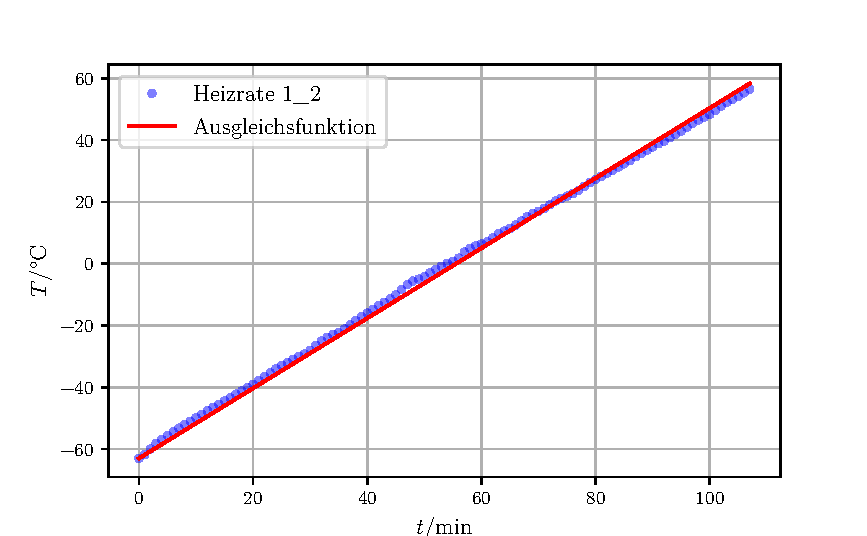
\includegraphics[width=\textwidth]{build/interpol_1_2.pdf}
  \caption{Messwerte und lineare Ausgleichsrechnung zur Bestimmung der tatsächlichen
  Heizrate für die Messreihe mit niedrigerer Heizrate.}
  \label{fig:heiz1}
\end{figure}
\begin{figure}
  \centering
  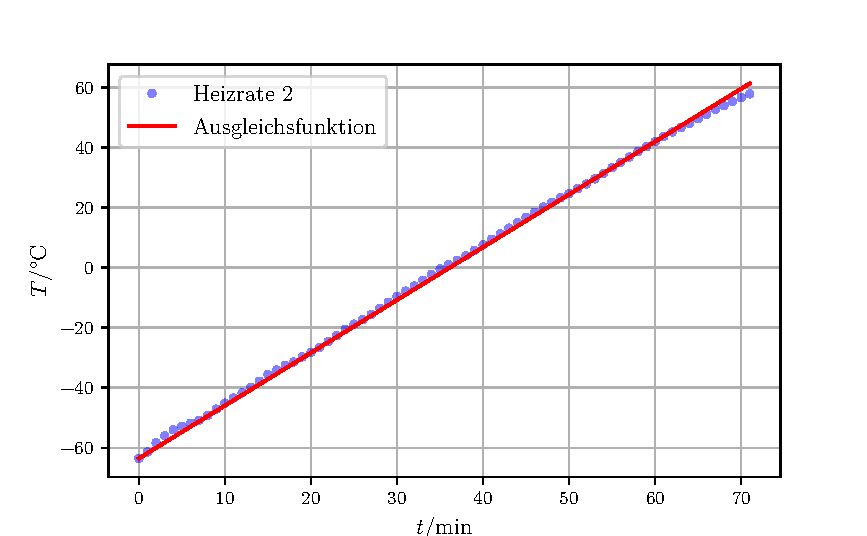
\includegraphics[width=\textwidth]{build/interpol_2.pdf}
  \caption{Messwerte und lineare Ausgleichsrechnung zur Bestimmung der tatsächlichen
  Heizrate für die Messreihe mit höherer Heizrate.}
  \label{fig:heiz2}
\end{figure}

\newpage
\subsection{Bestimmung und Abzug des Untergrundes}
\label{sec:untergrund}

Zur Bestimmung des Untergrundes müssen zunächst Werte für die Minima des Stroms per Hand gefunden
werden. Für die gefundenen Werte wird anschließend eine Ausgleichsrechnung der
Form
\begin{equation*}
  f(T)=a e^{bT} +c
\end{equation*}
durchgeführt\footnote{Durch eine weitere Parametrisierung des Exponenten wird der Fit nicht verbessert, da sich ein zusätzlicher Parameter auf die bereits gegebenen Parameter zurückführen ließe.}. Dabei ist der Wertebereich, der in der Ausgleichsrechnung verwendet wird,
manuell per Augenmaß bestimmt. Es wird dabei versucht, den Bereich vor starken Anstieg zum ersten Peak hin und den flachen Bereich hinter dem ersten Peak auszuwählen.
Es ergeben sich die Parameter
\begin{align*}
  a_1&=\SI{3.11(08)}{\pico\ampere}  \,,\\
	b_1&=\SI{0.0388(0013)}{\per\kelvin}  \,,\\
  c_1&=\SI{0.20(05)}{\pico\ampere}  \,,\\
  a_2&=\SI{4.79(33)}{\pico\ampere}  \,,\\
	b_2&=\SI{0.0286(0020)}{\per\kelvin}  \,,\\
  c_2&=\SI{-0.06(27)}{\pico\ampere}  \,.
\end{align*}
Die Ausgleichsfunktionen für den Untergrund, sowie die für die Ausgleichsrechnungen
verwendeten Werte sind in den Abbildungen \ref{fig:depol1} und \ref{fig:depol2} zu sehen.
Es ist grafisch ersichtlich, dass die Graphen der Ausgleichsfunktionen die verwendeten Werte gut beschreiben, was auch an den geringen relativen Unsicherheiten der multiplikativen Parameter $a_i$ und $b_i$ zu erkennen ist.
Außerdem sind in den Abbildungen die um den Untergrund bereinigten Daten dargestellt, mit denen auch im Folgenden weitergerechnet wird.

\begin{figure}
  \centering
  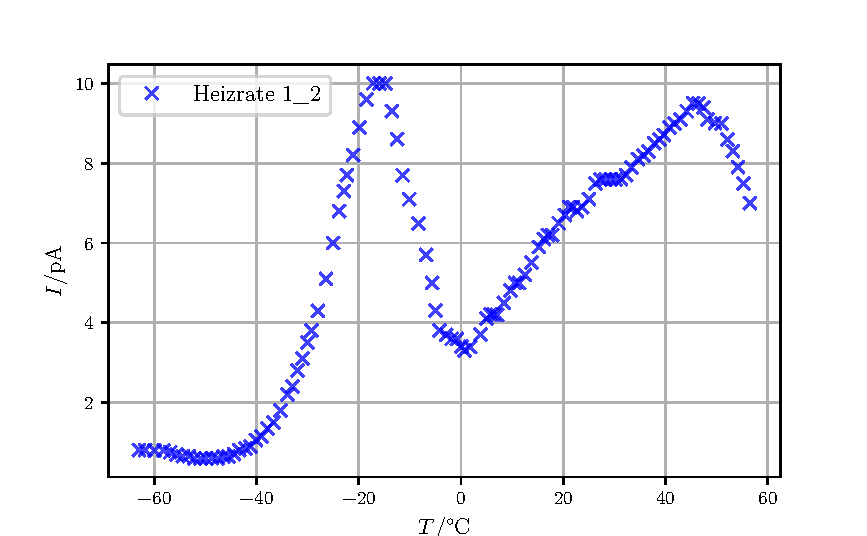
\includegraphics[width=\textwidth]{build/depolarisationskurve_1_2.pdf}
  \caption{Messwerte, sowie Ausgleichsrechnung für den Untergrund aus den markierten Werten
  und um den Untergrund bereinigte Daten für die Messreihe mit der niedrigeren Heizrate.}
  \label{fig:depol1}
\end{figure}
\begin{figure}
  \centering
  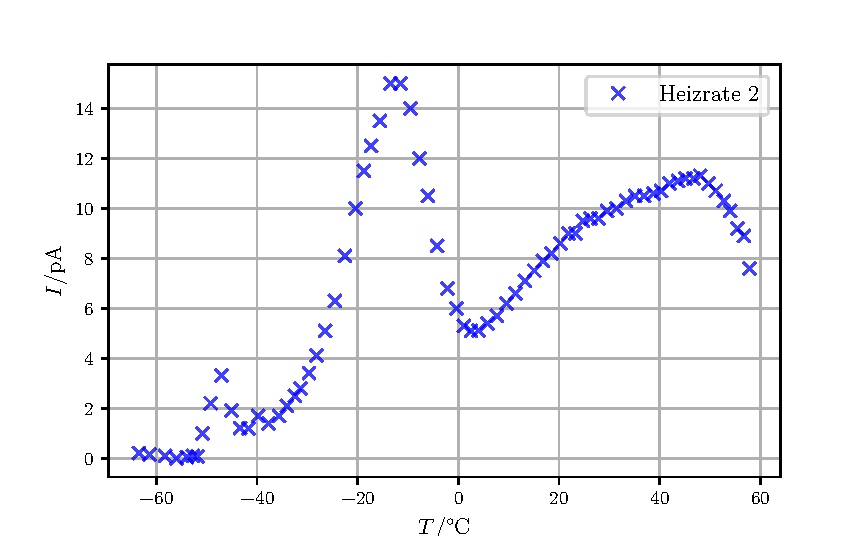
\includegraphics[width=\textwidth]{build/depolarisationskurve_2.pdf}
  \caption{Messwerte, sowie Ausgleichsrechnung für den Untergrund aus den markierten Werten
  und um den Untergrund bereinigte Daten für die Messreihe mit der höheren Heizrate.
	\cite{wieso haben wir hier dieses komische Maximum?.}}
  \label{fig:depol2}
\end{figure}

\newpage
\subsection{Bestimmung der Aktivierungsenergie über die Stromdichte}

Es wird die Näherung aus Gleichung \eqref{eqn:naeherung} in Form einer Stromstärke verwendet. Beide Seiten werden einheitenlos gemacht, indem durch Ampere geteilt wird \footnote{Der Übersichtlichkeit halber werden eigentlich einheitenlose Größen, mit denen auf diese Weise verfahren wurde, mit dem selben Buchstaben wie vorher bezeichnet.}. Es ist dann möglich, die Gleichung zu logarithmieren:
\begin{equation*}
  \ln(i(T))=-\frac{W}{k_B T} + \text{const} =a\cdot \frac{1}{T} +b  \,.
\end{equation*}
Dabei wird
Es wird nun $\ln(i(T))$ gegen $1/T$ aufgetragen und eine lineare Ausgleichsrechnung
durchgeführt. Dabei werden zunächst die Werte vom ersten Minimum bis zum erstem Maximum
des Depolarisationsstroms verwendet. Anschließend werden davon die Werte ausgewählt, die
noch einen annähernd linearen Verlauf zeigen. Die Werte für höhere Temperaturen werden
nicht berücksichtigt, da die oben genannte Näherung nur bei geringen
Temperaturen gültig ist.

Die Parameter
der Ausgleichsrechnungen ergeben sich zu
\begin{align*}
  a_1&=\SI{-7.3(4)e+3}{\kelvin} \,, \\
  b_1&=\SI{31.0(15)}{}  \,, \\
  a_2&=\SI{-8.8(7)e+3}{\kelvin} \,, \\
  b_2&=\SI{36.6(28)}{}  \,.
\end{align*}
Die Aktivierungsenergien können damit über $W=-ak_B$ zu
\begin{align*}
 W_1&=\SI{1.01(05)e-19}{\joule}= \SI{0.633(033)}{\eV}  \,, \\
 W_2&=\SI{1.22(010)e-19}{\joule}=\SI{0.76(06)}{\eV} \,.
\end{align*}
bestimmt werden. Der Literaturwert hierzu beträgt $W_{\text{lit}}=0{,}66\,$eV \cite{lit}. Davon weichen
die aus den Messwerten berechneten Werte um $-4{,}10\%$ für $W_1$ und $15{,}07\%$ für
$W_2$ ab.

Die Werte und die Ausgleichsrechnung sind in den Abbildungen \ref{fig:fit1} und
\ref{fig:fit2} dargestellt.

\begin{figure}
  \centering
  \includegraphics[width=\textwidth]{build/fit1.pdf}
  \caption{Messwerte und lineare Ausgleichsrechnung zur Bestimmung der Aktivierungsenergie mit dem Stromdichteansatz für
  die Messreihe mit der niedrigeren Heizrate.}
  \label{fig:fit1}
\end{figure}
\begin{figure}
  \centering
  \includegraphics[width=\textwidth]{build/fit2.pdf}
  \caption{Messwerte und lineare Ausgleichsrechnung zur Bestimmung der Aktivierungsenergie mit dem Stromdichteansatz für
  die Messreihe mit der höheren Heizrate.}
  \label{fig:fit2}
\end{figure}

\newpage
\subsection{Bestimmung der Aktivierungsenergie aus dem Polarisationsansatz}
\label{subsec:polarisation}

Zur Bestimmung der Aktivierungsenergie und der Relaxationszeit aus dem Polarisationsansatz wird
\begin{equation*}
	\ln\left(\frac{\int_T^{T^*}i(T') \symup{d}T'}{i(T) b_i}\right)
\end{equation*}
gemäß Gleichung \eqref{eqn:polAnsatz} gegen $1/T$ aufgetragen, wobei die charakteristische Relaxationszeit aus dem Logarithmus gezogen und als Konstante der Ausgleichsfunktion umgeschrieben wurde. Dabei sind die $b_i$ die in Kapitel \ref{sec:heiz}
berechneten Heizraten. Die Integration geschieht mithilfe der Trapezregel. Dabei sollte $j(T^*)\approx 0$ gelten. Es werden daher die Temperaturen
\begin{align*}
	T_1^* &=\SI{272.95}{\kelvin} \,, \\
	T_2^* &=\SI{275.65}{\kelvin}
\end{align*}
verwendet.
Anschließend werden Ausgleichsrechnungen der Form
\begin{equation*}
	\ln\left(\frac{\int_T^{T^*}i(T') \symup{d}T'}{i(T) b_i}\right) =\frac{W}{k_B T}+\ln(\tau_0)=\frac{A}{T}+B
\end{equation*}
durchgeführt, wobei die Anfangstemperaturen dieselben wie für die vorherigen Ausgleichsrechnungen sind. Es werden gezielt Messwerte herausgenommen, die entweder als Ausreißer anzusehen sind oder zwar zu einer Gerade ausgeglichen werden können, jedoch aufgrund von Fluktuationen in den Messwerten keine Information zur Ausgleichsrechnung beitragen (siehe Anfangsbereich in Abbildung \ref{fig:integral2}). Die Ausgleichsrechnungen sind in den
Abbildungen \ref{fig:integral1_2} und \ref{fig:integral2} grafisch dargestellt.
Des Weiteren werden für die Ausgleichsrechnung alle Wertepaare herausgenommen, für die das Argument des Logarithmus negativ wird. Diese Wertepaare sind in den Abbildungen nicht mehr dargestellt.

Die ermittelten Parameter betragen
\begin{align*}
  A_1&=\SI{9.95(24)e+03}{\kelvin} \,, \\
  B_1&=\SI{-32.7(10)}{}  \,, \\
  A_2&=\SI{1.095(030)e+04}{\kelvin} \,, \\
  B_2&=\SI{-36.5(12)}{}  \,.
\end{align*}

Die Aktivierungsenergien folgen dann aus den Anstiegen der
Ausgleichsgeraden über $W_i=A_i k_B$ zu
\begin{align*}
	W_1=\SI{1.373(033)e-19}{\joule}=\SI{0.857(021)}{\eV} \,, \\
	W_2=\SI{1.51(04)e-19}{\joule}=\SI{0.943(026)}{\eV} \,.
\end{align*}
Die Abweichungen vom oben genannten Theoriewert betragen hier
$29{,}88\%$ für $W_1$ und $42{,}95\%$ für $W_2$.

\begin{figure}
  \centering
  \includegraphics[width=\textwidth]{build/integral1_2.pdf}
  \caption{Messwerte und lineare Ausgleichsrechnung zur Bestimmung der Aktivierungsenergie mit dem Polarisationsansatz für
  die Messreihe mit der niedrigeren Heizrate.}
  \label{fig:integral1_2}
\end{figure}
\begin{figure}
  \centering
  \includegraphics[width=\textwidth]{build/integral2.pdf}
  \caption{Messwerte und lineare Ausgleichsrechnung zur Bestimmung der Aktivierungsenergie mit dem Polarisationsansatz für
  die Messreihe mit der höheren Heizrate.}
  \label{fig:integral2}
\end{figure}

\subsection{Bestimmung der Relaxationszeit}

Wie in Kapitel \ref{subsec:polAnsatz} erläutert, gilt der Zusammenhang
\begin{equation*}
	\tau_0=\frac{k_B T_{\text{max}}^2}{W b} e^{\left(-\frac{W}{k_B T_{\text{max}}}\right)} \,.
\end{equation*}
Aus den Aktivierungsenergien aus Kapitel \ref{subsec:polarisation} ergeben sich die Werte
\begin{align*}
	\tau_{0,1}=\SI{4.62(443)e-15}{\second} \,, \\
	\tau_{0,2}=\SI{1.03(121)e-16}{\second} \,.
\end{align*}
Während die Unsicherheit von $\tau_{0,2}$ größer als der Nominalwert ist, liegt die Unsicherheit von $\tau_{0,1}$ unter dem Nominalwert, allerdings ist die relative Unsicherheit mit $95{,}89\%$ sehr groß.
Die hohen Unsicherheiten entstehen dadurch, dass die Aktivierungsenergie $W$ in einer Exponentialfunktion eingeht, sodass der Fehler von $W$ verstärkt in $\tau_0$ eingeht.
Die Werte sind jedoch nicht allzu weit von dem Literaturwert von $\SI{4(2)e-14}{\second}$ \cite{lit} entfernt, der ebenso eine hohe Ungenauigkeit aufweist, wenn berücksichtigt wird, dass die Bestimmung von $\tau_0$ sehr sensitiv für Abweichungen in $W$ sind.
